%%=============================================================================
%% Methodologie
%%=============================================================================

\chapter{\IfLanguageName{dutch}{Methodologie}{Methodology}}
\label{ch:methodologie}

\section{Type onderzoek}
Het onderzoek beschreven in deze tekst is een \textbf{kwantitatief} onderzoek. Voor combinaties van het aantal auto's en het aantal reservaties zal het service level, de totale gebruiksduur van de auto's en de tijdsduur van de reservaties die niet konden doorgaan vergeleken worden. Vanuit een bedrijfsstandpunt is het interessant om het service level en de gebruiksduur van de auto's te maximaliseren voor een gegeven grootte van de vloot. Voor dit onderzoek wordt geopteerd voor een aanpak die zo dicht mogelijk aansluit bij de realiteit binnen het bestek van het onderzoek. In de stand van zaken werd een theoretische aanpak beschreven door middel van wachtrijtheorie. Een belangrijke stap hierbij is het bepalen van de parameter $\lambda$ van het Poisson-proces dat de aankomst van reservaties modelleert. Deze $\lambda$ is echter tijdsafhankelijk en niet hetzelfde voor elke dag van de week of periode van het jaar. In dit onderzoek worden simulaties uitgevoerd met een zelf-ontwikkelde simulatietool die historische reservaties van Partago gebruikt. De programmeercode van deze simulatietool is als bijlage opgenomen bij deze scriptie. Deze simulaties simuleren reëel reservatiegedrag van de Partago-gebruikers aangezien het gaat om echte reservaties. Verder in dit hoofdstuk wordt exact beschreven hoe deze simulaties zijn opgebouwd en welke stappen binnen elke simulatie uitgevoerd worden om tot numerieke waarden voor het service level en de gebruiksduur van de auto's te komen. 

\section{Eigenschappen van de dataset van reservaties} \label{eigenschappen-dataset}
Zoals hierboven vermeld zullen de reservaties in de simulaties komen uit een dataset van historische Partago reservaties. Voor er dieper wordt ingegaan op de simulaties zelf wordt deze dataset verkend. Met behulp van een rekenblad worden enkele interessante parameters berekend die een beter zicht geven hoe de reservaties verdeeld zijn en welke karakteristieken ze vertonen. 
\subsection{Aantal reservaties}
De dataset die gebruikt zal worden in dit onderzoek bestaat voor filtering uit alle reservaties gedaan op het Partago systeem van 1 januari 2019 tot en met 30 juni 2019. Voor filtering gaat dit om 7533 reservaties. Dit aantal wordt wel nog opgekuist vooraleer er simulaties mee gedaan zullen worden: reservaties niet uitgevoerd door Partago-coöperanten (bijvoorbeeld door het onderhoudsteam of door een partner bedrijf, welke onder een aparte regeling vallen) en geannuleerde reservaties worden verwijderd. Na het filteren zijn er nog een 4000-tal reservaties. Dit lijkt relatief weinig ten opzichte van de oorspronkelijke 7533. Een groot deel van deze oorspronkelijke 7533 reservaties bestaan uit reservaties die onder een aparte regeling vallen. Partago werkt samen met onder andere lokale overheden en energie-coöperaties om aan hun mobiliteitsbehoeften te voldoen. Deze reservaties, die vooral tijdens de werkuren vallen, werden allemaal weggefilterd aangezien deze lokale overheden en energie-coöperaties tijdens hun gebruik exclusief toegang hebben tot de auto's. Op die momenten worden de auto's dus niet meer gedeeld met de andere Partago-gebruikers. Deze reservaties zijn dus niet interessant voor dit onderzoek.
figuur \ref{grafiek:aantal-reservaties-per-week} geeft het aantal reservaties per week weer na filtering. Over de volledige 26 weken durende periode komt dit neer op een gemiddelde van 137 reservaties per week. Dit is echter een weinig zeggend cijfer, aangezien er in elke week een verschillend aantal auto's actief was. 
\begin{figure}[p]
	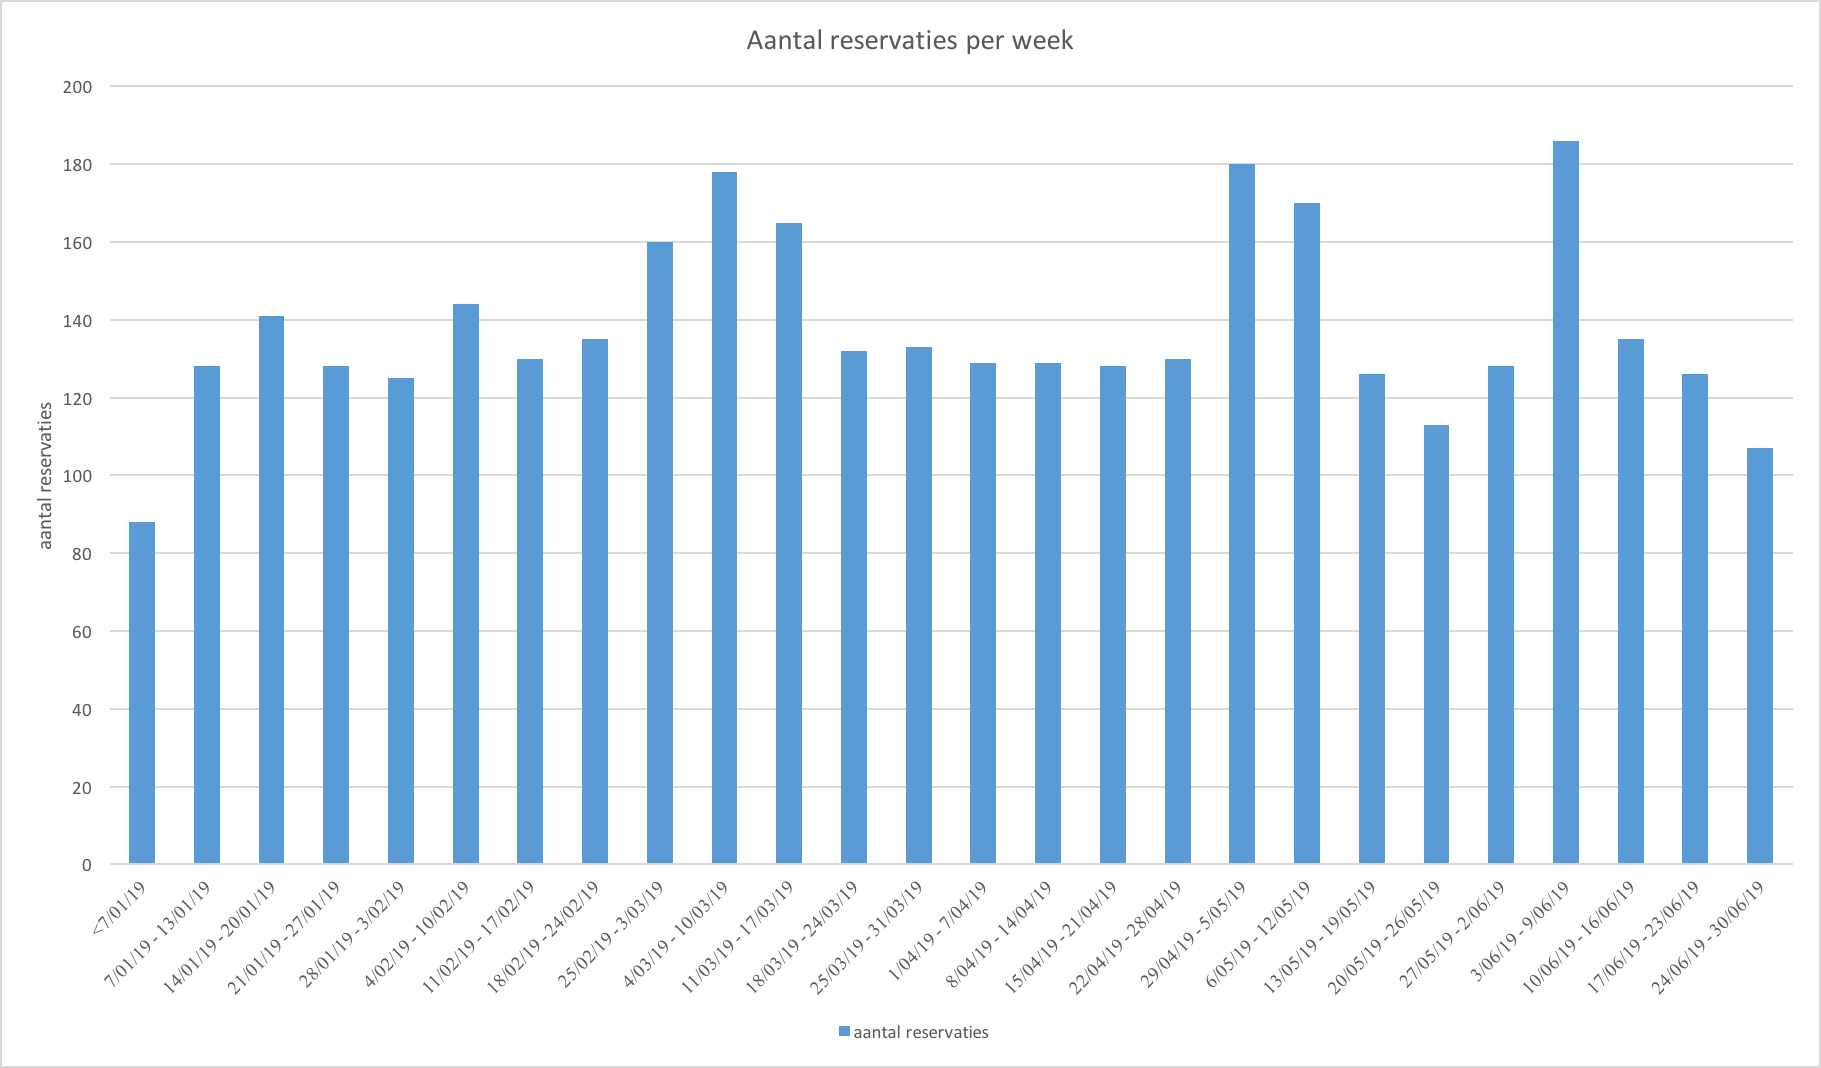
\includegraphics[width=\textwidth]{grafiek-aantal-reservaties-per-week.png}
	\caption[Aantal reservaties per week]{Histogram van het aantal reservaties per week na filtering}
	\label{grafiek:aantal-reservaties-per-week}
\end{figure}
Figuur \ref{grafiek:aantal-reservaties-per-week-per-auto} geeft het gemiddelde aantal reservaties per week per auto weer alsook het maximum aantal reservaties voor een auto dat voorkwam in die week. Over de gehele periode was er een gemiddelde van 2,9 reservaties per week per auto. De drukste week voor één enkele auto was 20 reservaties per week. 
\begin{figure}[p]
	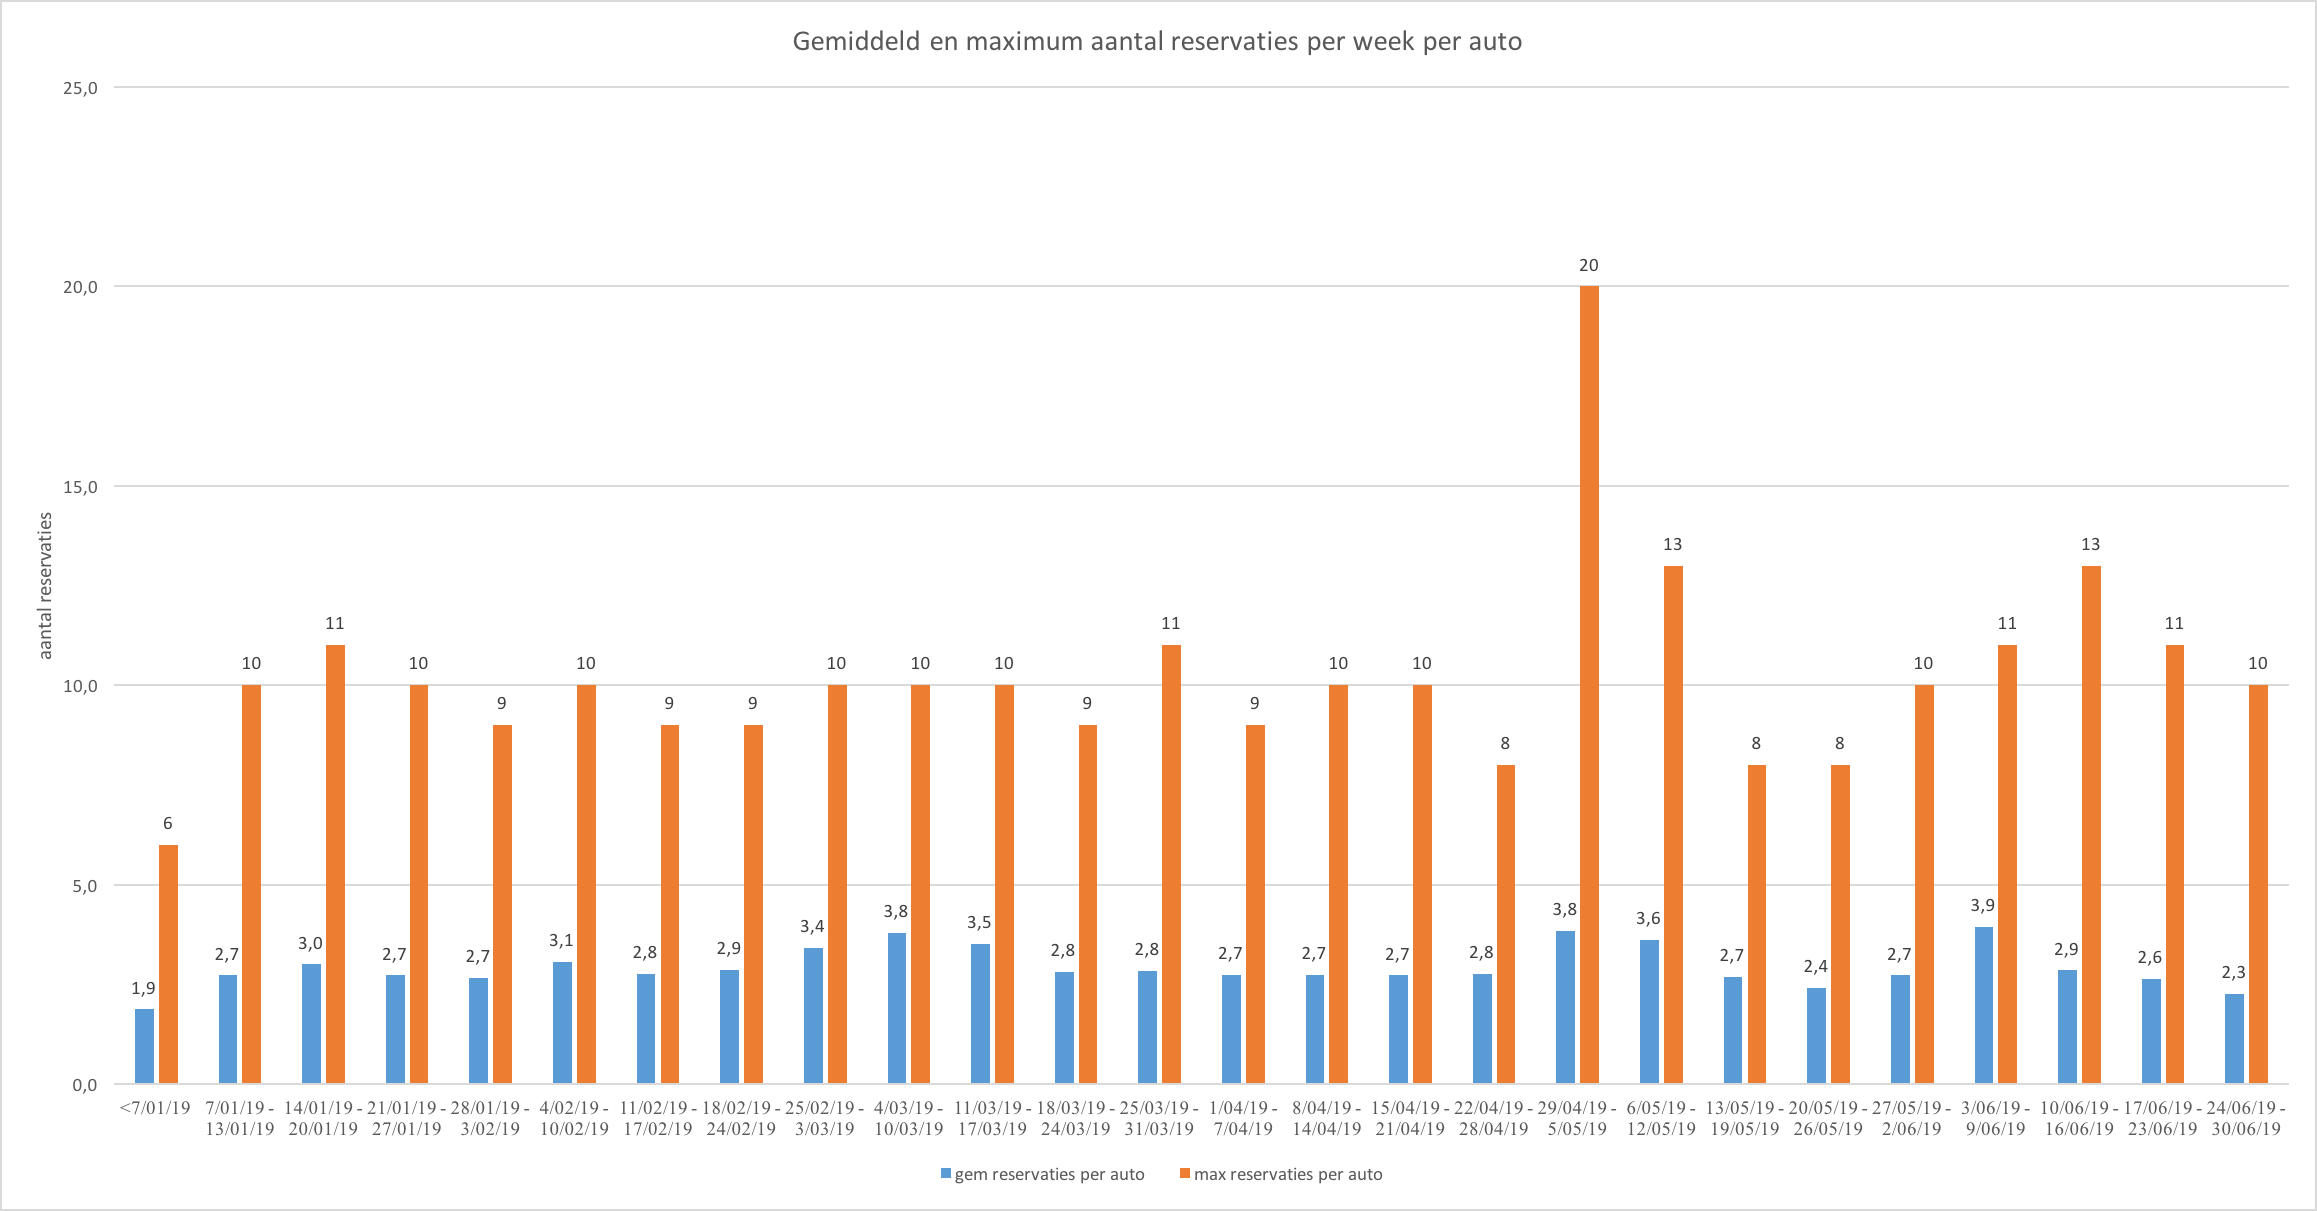
\includegraphics[width=\textwidth]{grafiek-gem-max-aantal-reservaties-per-week-per-auto.png}
	\caption[Gemiddelde en maximum per week per auto]{Histogram van het gemiddelde en maximum aantal reservaties per week per auto}
	\label{grafiek:aantal-reservaties-per-week-per-auto}
\end{figure}

\subsection{Verdeling reservaties}
Partago richt zich vooral op korte termijn gebruik van de auto's. Dit laat zich duidelijk blijken in figuur \ref{grafiek:gebruiksduur}.
De gemiddelde duur van een reservatie is 3 uur en 32 minuten. 80,08\% van de reservaties heeft een tijdsduur tussen de 0 en 5 uur. 4,73\% duurt 5 minuten of minder. Terwijl slechts 0,73\% langer dan 24 uur duurt. Deze zeer korte reservaties van minder dan 5 minuten kunnen verklaard worden doordat gebruikers een auto verplaatsen binnen de thuiszone van de auto: bijvoorbeeld om deze aan de laadpaal te hangen of om deze vlak voor de deur van hun huis te plaatsen. Een andere mogelijke verklaring is dat de gebruiker iets vergeten was in de auto en deze zeer kort reserveert om de deuren te kunnen openmaken.  
\begin{figure}[p]
	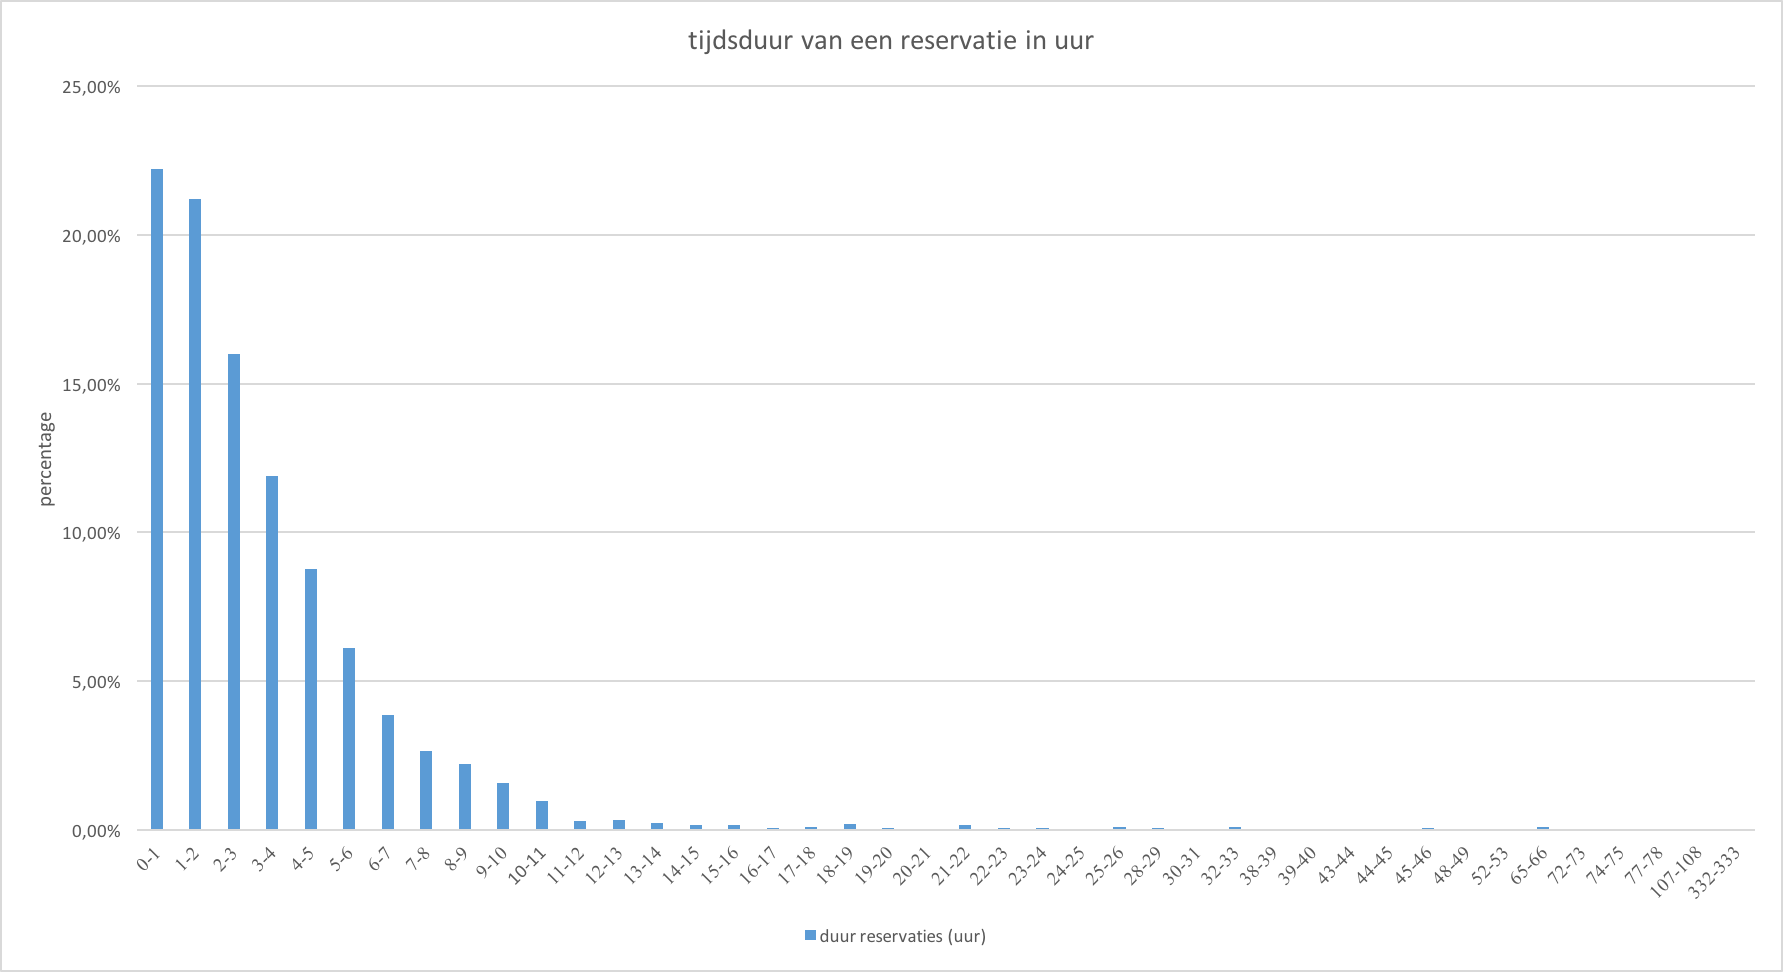
\includegraphics[width=\textwidth]{grafiek-tijdsduur-reservaties.png}
	\caption[Duur van een reservatie]{Histogram van de duur van een reservatie}
	\label{grafiek:gebruiksduur}
\end{figure}
Figuur \ref{grafiek:weekdag} toont een histogram van de reservaties gegroepeerd per dag van de week. Maandag, dinsdag, donderdag en vrijdag zijn relatief gelijk. De drukste dag is over duidelijk zaterdag met 20,71\% van alle reservaties. Ook woensdag en zondag vertonen een kleine verhoging ten opzichte van de andere weekdagen.
\begin{figure}[p]
	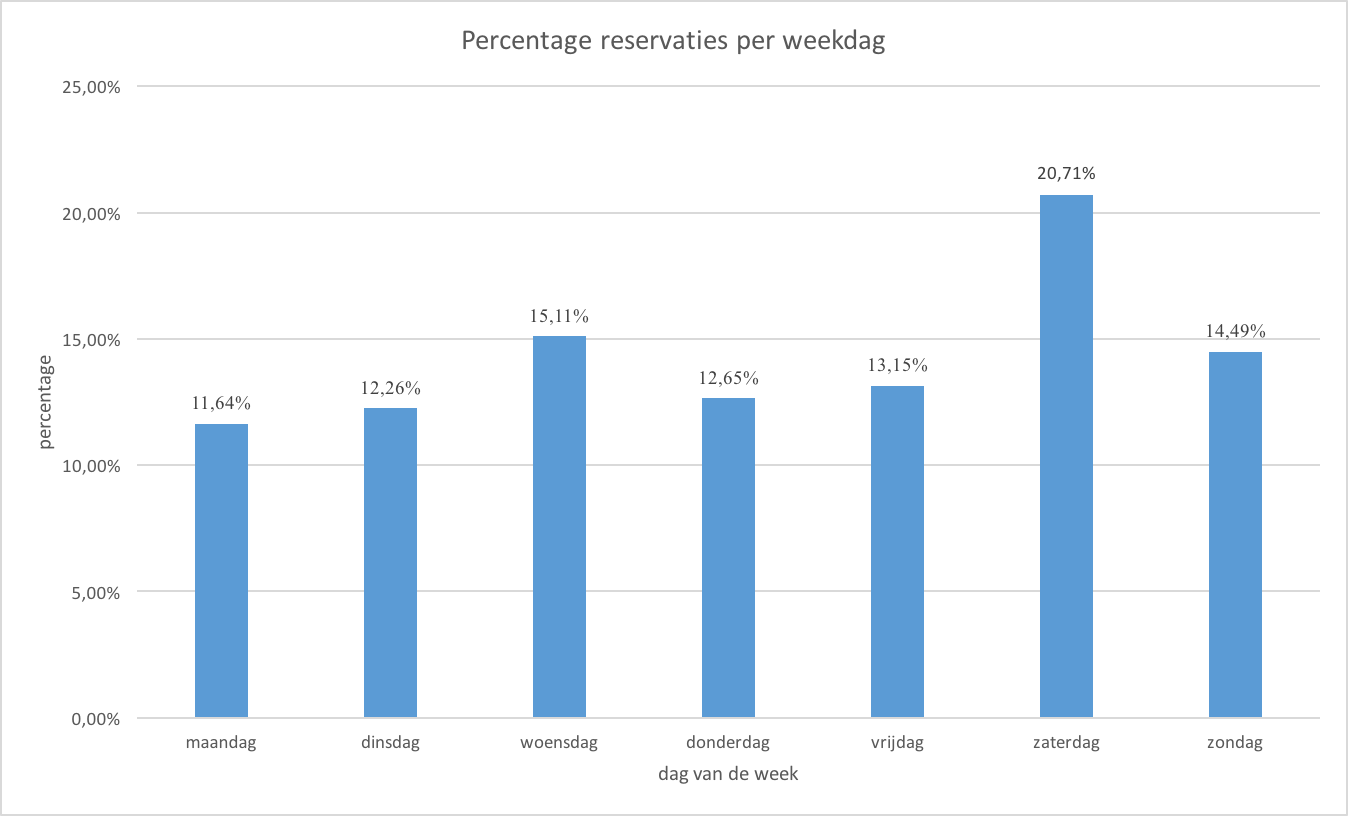
\includegraphics[width=\textwidth]{grafiek-weekdag-reservaties.png}
	\caption[Dag van de week van een reservatie]{Histogram van de reservaties verdeelt per weekdag}
	\label{grafiek:weekdag}
\end{figure}
Ook figuur \ref{grafiek:starttijd} toont geen grote verrassingen. De meeste reservaties starten tussen 8 uur 's ochtends en 20 uur 's avonds (91,69\%).
\begin{figure}[p]
	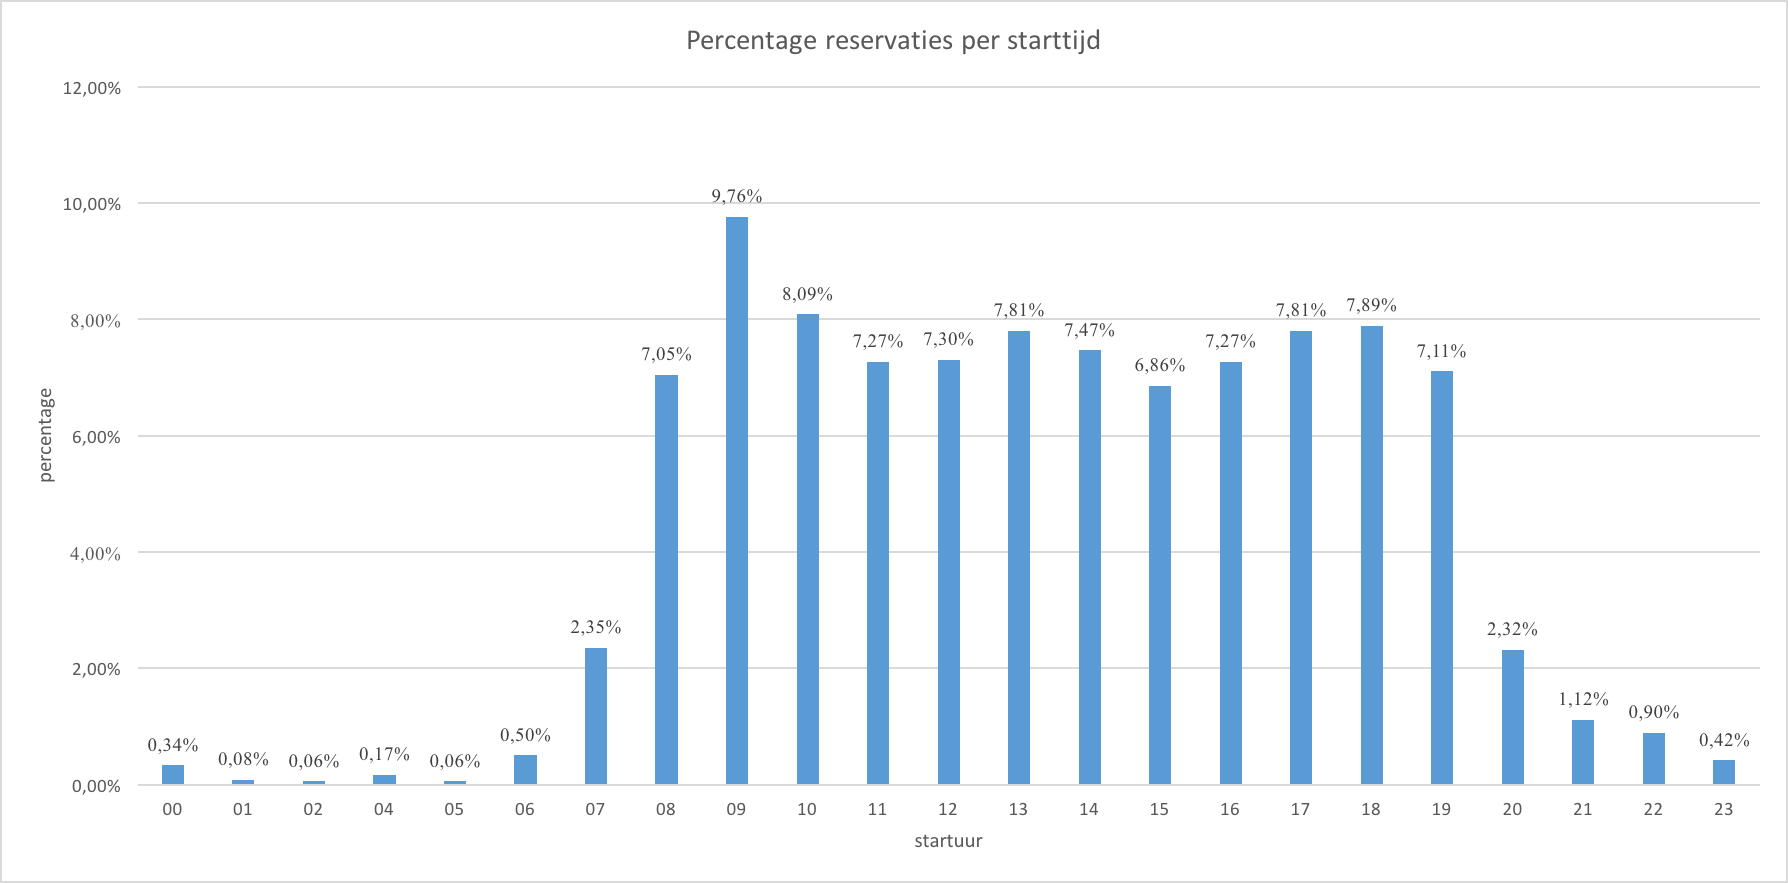
\includegraphics[width=\textwidth]{grafiek-starttijd.png}
	\caption[Starttijd van een reservatie]{Histogram van de startijd van de reservaties}
	\label{grafiek:starttijd}
\end{figure}


\section{Opzet van een simulatie} \label{opzet-simulatie}
\subsection{Doel}
Tijdens de simulatie wordt er getracht tweemaal een toewijzing te doen van de beschikbare auto's aan de reservaties. Eenmaal zal deze toewijzing gebeuren op een eenvoudige manier en eenmaal zal deze toewijzing gebeuren door het oplossen van het corresponderende Constraint Satisfaction Problem (zie verder en in hoofdstuk \ref{ch:stand-van-zaken}). Voor beide toewijzingen wordt het service level, de tijd dat de auto's actief waren en de tijd van reservaties die niet konden doorgaan omdat er geen auto beschikbaar was berekend. Een algoritme om CSP's op te lossen geeft een oplossing voor het probleem, maar niet per se steeds dezelfde (zie ook hoofdstuk \ref{ch:stand-van-zaken}). Voor verschillende simulaties met gelijke parameters zullen er dus verschillende waarden voor het service level en de tijd dat de auto's actief waren bekomen worden. Een simulatie wordt daarom meermaals uitgevoerd om dan een gemiddeld service level, een gemiddelde actieve tijd van de auto's en een gemiddelde tijd van reservaties die niet konden doorgaan te berekenen.

\subsection{Karakteristieken}
Eén enkele simulatie wordt gekarakteriseerd door waarden van de volgende grootheden:
\begin{itemize}
	\item \textbf{Aantal reservaties in de simulatie:}
	Het aantal reservaties is een maat voor de drukte op het systeem. Het aantal gebruikers van het systeem zou hier geen goede maat voor zijn, weinig gebruikers kunnen immers ook relatief veel reservaties maken. Veel reservaties betekent een grote drukte op het systeem, weinig reservaties betekent een kleine drukte. Uiteraard kunnen overlappende reservaties niet van dezelfde persoon afkomstig zijn. De reservaties gebruikt in de simulatie zijn bestaande historische reservaties van Partago.
	\item \textbf{Aantal auto's:}
	Tijdens de simulatie zullen er toewijzingen gebeuren van de auto's aan de reservaties. Meer auto's beschikbaar in de fictieve zone zal het service level onmiddellijk doen toenemen. Voor eenzelfde aantal reservaties zullen meer reservaties kunnen doorgaan als er meer auto's beschikbaar zijn. 
	\item \textbf{Aantal weken:}
	Elke simulatie stelt een fictieve reserveringsperiode voor van een aantal weken. Tijdens dit onderzoek wordt deze parameter vastgehouden op \textbf{4 weken}. Tijdens elke simulatie zullen we dus een periode van vier weken simuleren. 
\end{itemize} 

\subsection{Stappen binnen een simulatie}
Binnen één enkele simulatie worden de volgende stappen ondernomen
\begin{enumerate}
	\item Definiëren van de karakteriserende parameters
	\item Historische Partago reservaties ophalen
	\item Een dataset van reservaties genereren op basis van de historische gegevens voor de gedefinieerde periode
	\item Een eenvoudige toewijzing doen van auto's op de reservaties uit de dataset
	\item Een toewijzing doen van auto's op de reservaties uit de dataset met behulp van een CSP oplosalgoritme 
	
\end{enumerate}
Op elk van deze stappen wordt dieper ingegaan in de komende secties van dit hoofdstuk. 

\section{Definiëren van de karakteriserende parameters} \label{karakteriserende-parameters}
\subsection{Aantal reservaties}
De kennis die verworden werd in \ref{eigenschappen-dataset} wordt gebruikt om de karakteriserende parameters van een simulatie te definiëren. Het gemiddelde aantal reservaties per week per auto werd reeds berekend voor de periode van 1 januari 2019 tot en met 30 juni 2019 en kwam uit op gemiddeld 2,9 reservaties per week per auto die zijn doorgegaan. Dit getal houdt enkel rekening met reservaties die effectief zijn doorgegaan en die gedaan zijn door echte gebruikers (dus bijvoorbeeld niet door het onderhoudsteam). Hoeveel reservaties niet konden doorgaan weet het Partago systeem niet. Uit dit gemiddelde kan wel het vermoeden afgeleidt worden dat het Partago systeem momenteel een niet druk systeem is, de vloot relatief onbezet en nagenoeg een service level van 100\% bereikt zal worden. Het aantal reservaties is discreet, het bovenvermelde gemiddelde wordt afgerond tot 3. Voor de uit te voeren simulaties zal de drukte op het systeem opgedreven worden: maal factor 3, factor 5 en factor 10. Het aantal reservaties zal dus variëren van 9 reservaties per week per auto tot 30 reservaties per week per auto. Er wordt gekozen om te starten met een factor 3 aangezien voor factor 2 er gemiddeld 6 reservaties per week per auto zijn. Dit is nog steeds, gemiddeld gezien, nog niet 1 reservatie per dag waardoor een toewijzingsalgoritme niet aan de orde is.
\subsection{Aantal auto's}
Het aantal auto's in een simulatie is afhankelijk van het gekozen aantal reservaties en de drukte die hier mee overeenstemt. Zo is het niet interessant om op een niet druk systeem een simulatie uit te voeren met 50 auto's. Dit is geen reële situatie. Binnen het huidige systeem van Partago telt een zone 1, 2 of 3 auto's. Er wordt dus in de eerste plaats gekozen voor een relatief klein aantal auto's tijdens de simulaties aangezien dit het dichtste aansluit bij hoe Partago momenteel georganiseerd is. Naarmate het aantal auto's stijgt, hoe complexer het probleem. Bij meer complexere problemen wordt een grotere winstmarge verwacht van de toewijzing met behulp van CSP ten opzichte van de eenvoudige toewijzing. Er wordt gekozen om voor elke druktegraad een simulatie uit te voeren met 3 en 5 auto's. Voor de drukste systemen wordt ook een simulatie uitgevoerd met 10 auto's.
\subsection{Aantal weken}
Deze parameter wordt vastgehouden op 4 weken. Deze keuze is arbitrair. De simulaties over een langere periode laten lopen zou de rekentijd aanzienlijk verhogen en weinig meerwaarde bieden. Zoals eerder vermeld wordt een simulatie met een set van parameters meermaals uitgevoerd om gemiddelden te kunnen berekenen. Het lijkt misschien logisch om deze parameter groter te nemen, maar over langere periodes spelen seizoensgebonden factoren, zoals schoolvakanties, mee een grote rol en deze worden niet opgenomen in dit onderzoek.
\subsection{Uit te voeren simulaties}
De simulaties die uitgevoerd zullen worden worden weergegeven in volgende tabel:
\begin{center}
	\label{tab:parameters}
	\begin{tabular}{ | l | l | l | p{3cm} |}
		\hline
		Aantal reservaties & Aantal auto's & Druktegraad & Aantal weken \\ \hline
		108 & 3 & 9 reservaties/week/auto & 4 \\ \hline
		180 & 5 & 9 reservaties/week/auto & 4 \\ \hline
		180 & 3 & 15 reservaties/week/auto & 4 \\ \hline
		300 & 5 & 15 reservaties/week/auto & 4 \\ \hline
		360 & 3 & 30 reservaties/week/auto & 4 \\ \hline
		600 & 5 & 30 reservaties/week/auto & 4 \\ \hline
	\end{tabular}
\end{center} 

\section{Partago reservaties ophalen} \label{partago-reservaties-ophalen}
De dataset van reservaties die gegenereerd wordt is gebaseerd op bestaande reservaties uit het verleden gedaan op het systeem van Partago. Dit geeft als voordeel dat de dataset een reëel karakter zal vertonen en dus dicht aansluit op werkelijk reserveringsgedrag. Voor dit onderzoek worden historische gegevens van Partago van 1 januari 2019 tot en met 30 juni 2019 gebruikt. Voor eenvoud van de simulaties gebruiken we enkel reservaties die langer zijn dan 5 minuten en korter zijn dan 24 uur. Uit \ref{eigenschappen-dataset} weten dat slechts een klein aandeel van de dataset hierbuiten zal vallen, respectievelijk 4,73\% en 0,73\%.

\section{Dataset van reservaties genereren} \label{dataset-genereren}
Uit de gefilterde lijst van Partago reservaties zal een simulatie-specifieke dataset van reservaties gegenereerd worden voor een periode van het gedefinieerde aantal weken. In dit onderzoek zal elke dataset dus bestaan uit reservaties voor 4 weken. De parameter ``aantal reservaties`` zal bepalen hoeveel reservaties zich in de dataset bevinden. Dit aantal wordt willekeurig geselecteerd uit de historische Partago reservaties en gemapt op een willekeurige week in de dataset (week1, week2, week3 of week4), maar met behoudt van de dag van de week. Reservatiegedrag op een dinsdag is immers niet hetzelfde als reservatiegedrag op een zaterdag. Deze informatie mag  niet verloren gaan tijdens het mappen. Aangezien de reservaties willekeurig geselecteerd worden zullen de reservaties per dag in een willekeurige volgorde staan en dus niet in chronologische volgorde. Dit is eveneens de volgorde waarmee de reservaties toekomen bij het systeem. Figuur \ref{fig:visuele-voorstelling-dataset} is een visuele voorstelling van een eenvoudige dataset van 2 weken met 52 reservaties. Figuur \ref{fig:visuele-voorstelling-dag-dataset} toont in detail woensdag uit de dataset van figuur \ref{fig:visuele-voorstelling-dataset}. Merk op dat de reservaties niet in chronologische volgorde toekomen bij het systeem.
\begin{figure}[h]
	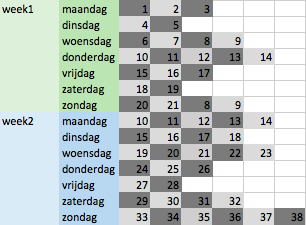
\includegraphics{dataset.png}
	\caption[visuele voorstelling dataset]{visuele voorstelling van een dataset van 2 weken met 52 reservaties}
	\label{fig:visuele-voorstelling-dataset}
\end{figure}
\begin{figure}[h]
	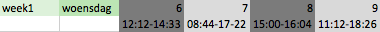
\includegraphics{dataset-detail.png}
	\caption[visuele voorstelling van 1 dag]{visuele voorstelling van 1 dag uit de dataset}
	\label{fig:visuele-voorstelling-dag-dataset}
\end{figure}
\section{Eenvoudige toewijzing} \label{eenvoudige-toewijzing}
Voor elke reservatie in de dataset zal geprobeerd worden een beschikbare auto toe te wijzen. Met de implementatie van de eenvoudige toewijzing wordt getracht het huidige reservatiemechanisme te modelleren. De volgorde dat de reservaties in de dataset zitten is de volgorde waarmee de reservaties toekomen bij het systeem. De eenvoudige toewijzing is ook weergegeven in het diagram in figuur 3.2. Alle reservaties in de dataset worden overlopen startend met de eerste reservatie op week1 maandag en eindigend, in dit onderzoek, bij week4 op zondag. De daglijst van reservaties wordt overlopen in de volgorde dat de reservaties in de lijst staan. Uit de beschikbare auto's wordt telkens een willekeurige auto gekozen tot een auto gevonden wordt die nog niet eerder bekeken werd voor deze reservatie. Indien de auto deze reservatie kan vervullen wordt de auto toegewezen aan de reservatie, indien deze auto reeds bezet is tijdens het tijdsinterval van de reservatie wordt er opnieuw een willekeurige auto gekozen die nog niet eerder geprobeerd werd. Indien alle auto's geprobeerd zijn, maar er was geen toewijzing mogelijk kan deze reservatie niet doorgaan en wordt deze toegevoegd aan de lijst van niet-geserveerde reservaties. Dit proces wordt herhaald voor alle reservaties. Elke succesvolle toewijzing wordt ook opgeslagen. Nadat alle reservaties overlopen zijn kan het service level uitgerekend worden door het aantal reservaties dat kon doorgaan te delen door het totaal aantal reservaties in de dataset. 
\section{Toewijzing met behulp van een CSP} \label{csp-toewijzing}
Voor elke reservatie in de dataset zal opnieuw geprobeerd worden een beschikbare auto toe te wijzen, maar deze keer zal voor elke dag in de dataset een Constraint Satisfaction Problem opgesteld worden en zal getracht worden dit probleem op te lossen (zie ook stand van zaken). Het toewijzen met behulp van een CSP is ook weergegeven in het diagram in figuur 3.3. Met deze aanpak wordt er vanuit gegaan dat alle reservaties voor een bepaalde dag gekend zijn voor aanvang van de eerste reservatie. De toegewezen auto voor een reservatie kan dus nog wijzigen naarmate het CSP opgelost wordt. Alle reservaties worden opnieuw overlopen startend bij week1 maandag en eindigend bij week4 zondag. De daglijst van reservaties wordt overlopen in de volgorde dat de reservaties in de lijst staan. Eén voor één worden de reservaties toegevoegd aan het CSP. Na elke toevoeging wordt het CSP opnieuw opgelost. Indien er door het toevoegen van een reservatie geen consistente oplossing meer gevonden kan worden, met andere woorden niet elke reservatie kreeg een auto toegewezen, wordt de reservatie terug verwijderd uit het probleem en toegevoegd aan de lijst van niet-geserveerde reservaties. Dit proces wordt herhaald voor elke reservatie van die dag. De uiteindelijke toewijzing voor die dag wordt ook opgeslagen om de tijd dat de auto's actief waren te kunnen berekenen. Voor elke dag in de dataset wordt gestart met een nieuw, leeg CSP. Nadat alle dagen overlopen zijn kan het service level uitgerekend worden door het aantal reservaties dat kon doorgaan te delen door het totaal aantal reservaties in de dataset. Voor het oplossen van het CSP wordt gebruik gemaakt van een externe softwarebibliotheek.





